\documentclass[twocolumn,amsmath,amssymb,floatfix]{article}

\usepackage{graphicx}% Include figure files
\usepackage{color}
\usepackage{dcolumn}% Align table columns on decimal point
\usepackage{bm}% bold math
\usepackage{amsmath}
\usepackage{hyperref}
\usepackage{comment}
\definecolor{clr1}{rgb}{0.2,0.8,0.0}
\definecolor{clr2}{rgb}{1,0.2,0.2}
\definecolor{clr3}{rgb}{1,0.6,0.1}
\usepackage{textcomp}
\usepackage{siunitx}


\hypersetup{
    bookmarks=true,         % show bookmarks bar?
    unicode=false,          % non-Latin characters in AcrobatÕs bookmarks
    pdftoolbar=true,        % show AcrobatÕs toolbar?
    pdfmenubar=true,        % show AcrobatÕs menu?
    pdffitwindow=false,     % window fit to page when opened
    pdfstartview={FitH},    % fits the width of the page to the window
    pdftitle={My title},    % title
    pdfauthor={Author},     % author
    pdfsubject={Subject},   % subject of the document
    pdfcreator={Creator},   % creator of the document
    pdfproducer={Producer}, % producer of the document
    pdfkeywords={keyword1} {key2} {key3}, % list of keywords
    pdfnewwindow=true,      % links in new window
    colorlinks=true,       % false: boxed links; true: colored links
    linkcolor=blue,          % color of internal links (change box color with linkbordercolor)
    citecolor=blue,        % color of links to bibliography
    filecolor=blue,      % color of file links
    urlcolor=blue           % color of external links
}
%\usepackage{showlabels}


\begin{document}


\title{Darcy 02 notes}
\author{Florencia Falkinhoff}
% \affiliation{LPENS}
\affiliation{IFPEN}
% \email{florencia.falkinhoff@ens-lyon.fr}

\author{Alexandre Ponomarenko}
\author{Mica}
\author{Romain}
% \affiliation{LPENS}

\author{Jean-Lou Pierson}
\author{Lionel Gamet}
\affiliation{IFPEN}
\date{\today, version 01}

\begin{abstract}
%Vulnerability to cavitation defines the range of water potentials at which plants can function. Below a certain tension, xylem conduits can become air-filled and gas may spread throughout the wood thus reducing t
\end{abstract}

%\pacs{
%47.63.Jd, % Microcirculation and flow through tissues
%92.40.Oj  %Eco-hydrology; plant ecology,
%}
\maketitle

\section{Details for the experiement shown in the abstract}

frames per second: $780$fps.\\
exposure time: $1282$  $\mu$s\\


\section{Introduction}
introduction introduction introduction

\subsection{Discussion Vincent}

fraction volumique tas de billes molles.?

\begin{figure}
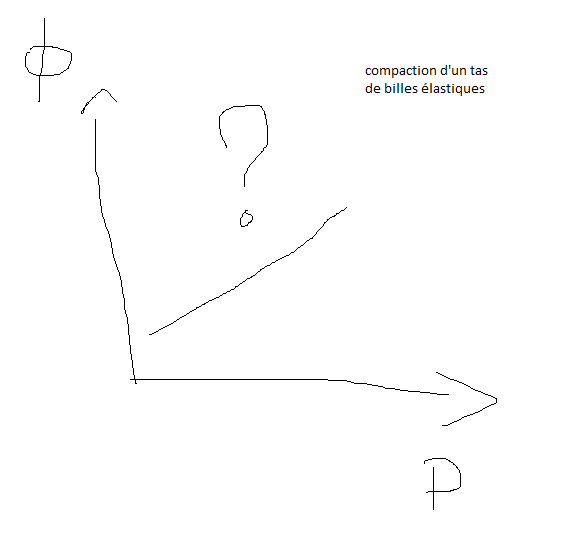
\includegraphics[height=8cm]{figures/elasticBeadsStack_VolumicFraction.png}
\caption{Figure idea about the volumic fraction of an elastic stack of beads.}
\label{fig:volFrac_elasticStac}
\end{figure}

\subsection{Notes pour discussion avec Romain Volk}

\begin{itemize}
    \item achat billes pour remplir la colonne.
    \item Analyse 3D.
    \item Analyse PTV.
    \item Qualité caméra VS qualité téléphone portable?
\end{itemize}


\begin{figure}
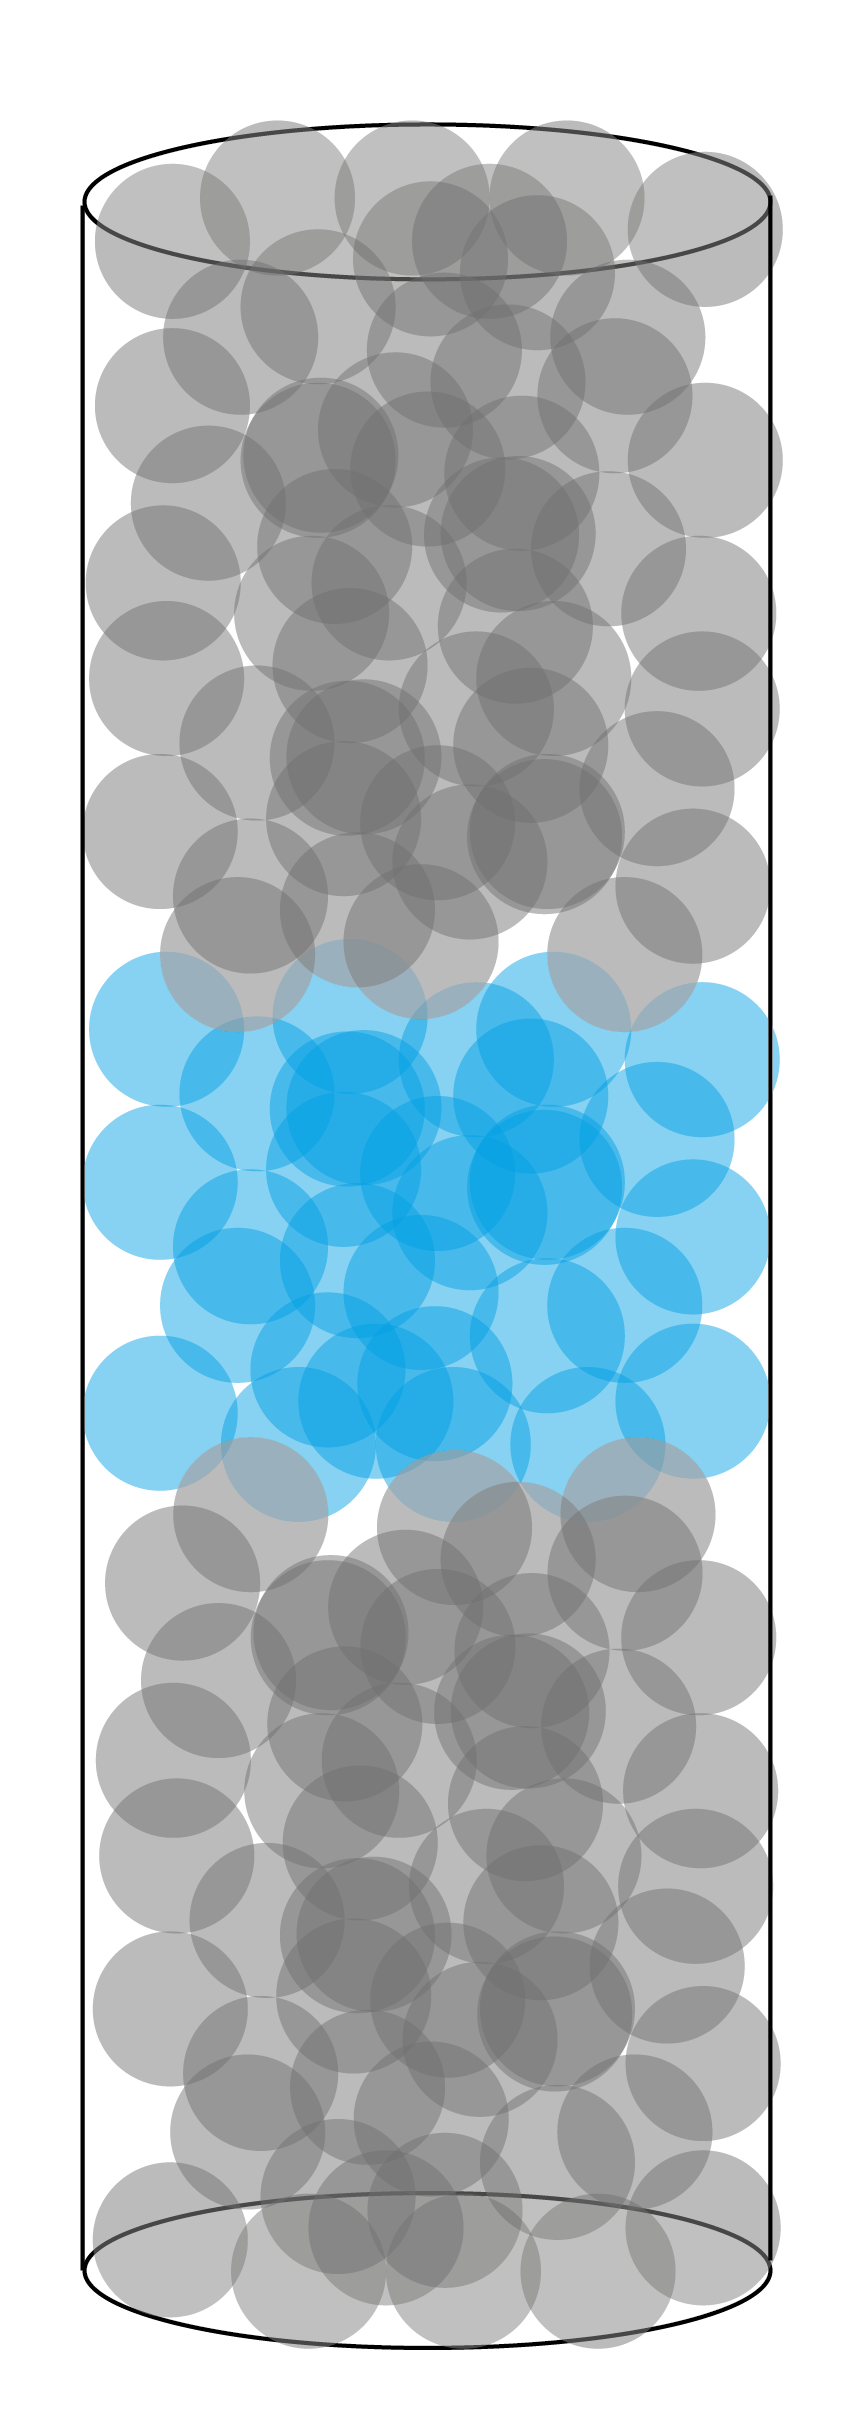
\includegraphics[height=8cm]{figures/beadsStack.png}
\caption{beads}
\label{fig:beads}
\end{figure}

%\begin{figure}
%\includegraphics[width=8cm]{figures/SEM-1.eps}\vspace{-2.2cm}\hspace{-3.2cm}
%\includegraphics[width=3cm]{./makefig0/SEM/SEM-2.eps}\vspace{2.2cm}\\
%\caption{}
%\end{figure}

% * <fulton.rockwell@gmail.com> 2017-05-29T12:21:57.317Z:
% 
% Do we need to invoke capillary sealing here? Or can we just note that at some critical pressure air can invade across the membrane?
% 
% ^.
\begin{equation}
p^{*}\approx \frac{2\gamma}{r^{*}}.\label{eq:ppit}
\end{equation}

\section{TODO list}

- gcc compilateur c++
- mpi for parallelisation

\subsection{Calibration with two level target}

Adapt David Dumond 4DPTV program to the new scale target.\\

Remarks: for the calculation of the spatial transformation from image points (pimg) to 2D postition in real space (pos2D), the code uses the function $T3rw2px  = fitgeotrans(pimg,pos2D,'polynomial',3);$, if there is not enough points it reports : " Error using images.geotrans.PolynomialTransformation2D (line 162)
At least 10 non-collinear points needed to infer polynomial transform. " . To deal with that, a possibility is to set the polynomial degree to $2$ instead of $3$.\\

Depending on the face you look at, the square is on a up line or on a down line. On figure (\ref{fig:caltarget}), the square is on an UP line.

The calibration target has $23$ lines. The DOWN lines have $12$ circles. The UP lines have 11 circles. There are two aditional elements: a square on line $11$ and a triangle on line $12$. There is a total of $143$ circles on DOWN lines and $121$ circles on UP lines plus a square on line $11$ and a triangle on line $12$. \\

Worflow for doing the calibration with this special target: $20$\textdegree{}C or $44.9^\circ$C \SI{44.9}{\celsius}

\begin{figure}
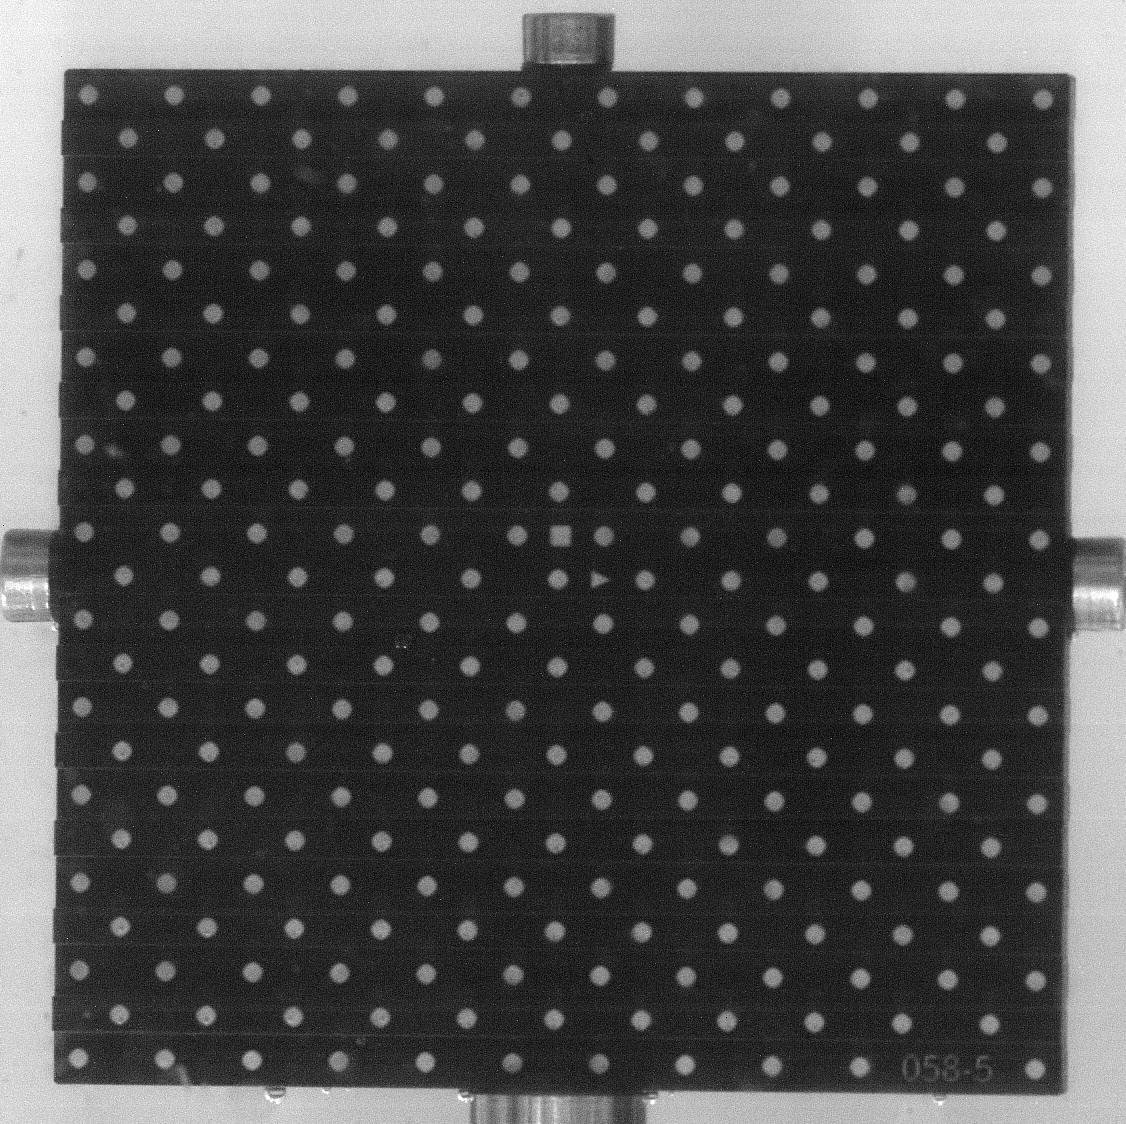
\includegraphics[height=8cm]{figures/calibrationTarget.png}
\caption{calibration target}
\label{fig:caltarget}
\end{figure}


%%%%%%%%%%%%%%%%%%%%%%%%%%%%%%%%%%%%%%%%%%%%
%%%%%%%%%%%%%%%%%%%%%%%%%%%%%%%%%%%%%%%%%%%%
%%%%%%%%%%%%%%%%%%%%%%%%%%%%%%%%%%%%%%%%%%%%
\section{Material and Methods}

\subsection{4D PTV}

The code is on github \href{https://github.com/turbulencelyon/4d-ptv}{4D-ptv on git} and the documentation on \href{https://4d-ptv.readthedocs.io/en/latest/}{read the docs}. 


I install VisualStudioCode, and add C++ tools following this tutorial \href{https://code.visualstudio.com/docs/languages/cpp}{Visual Studio Code C++}. I can compile C++ code.

Installing gcc. I used tips from here: \href{https://www.cs.odu.edu/~zeil/cs250PreTest/latest/Public/installingACompiler/}{link} but I downloaded MinGCW from \href{https://sourceforge.net/projects/mingw-w64/files/Toolchains\%20targetting\%20Win32/Personal\%20Builds/mingw-builds/installer/mingw-w64-install.exe/download}{download MinGW} as indicated on VSCode infos: \href{https://code.visualstudio.com/docs/cpp/config-mingw}{VSCode MinGW}

Change drive in command prompt. To go to D: cd /d D:
Instead of 'make', use 'mingw32-make'

Install hf5++ , good guide \href{https://accserv.lepp.cornell.edu/svn/packages/hdf5/release_docs/INSTALL}{here} and maybe also \href{http://hdf-forum.184993.n3.nabble.com/Trouble-compiling-with-h5c-td4027367.html}{here} and \href{https://stackoverflow.com/questions/60271865/compiling-hdf5-source-with-g}{here}

\subsubsection{PSMN}

./STM -i "./test/rays.dat" -o "./test/" -f 10 -c 2 -d 0.2 -s 1 -m 2 -x 400 -y 400 -z 400 -b -3 3 -3 3 1 5 --hdf5 >> rays.log


\subsection{Sketch plugging the two cameras together}

Shut off all Windows fire walls\\
terminal:\\
ping 100.100.111.52\\
ping 100.100.118.227\\

\subsection{index matching beads}
\subsubsection{Hydrogel beads}
There are three hydrogel beads names $1$, $2$ and $3$.
Order of preference: $1$, $3$, $2$.

About hydrogel beads $2$. They come in pinky pockets named Jelly-Beads, containing $5.1$g of beads that means $\sim300$ beads
\subsection{Flow Meter}

\subsection{solenoid valve: Burkert}

\subsection{tunings for electrovannes}

note from 2021 01 15\\
electrovanne\\
ancien réglage (DARCY 01):\\
low  564 \\
high 665\\


\subsection{3D printer}

\subsection{HDR image from bracketing exposure time image sequence}

https://docs.opencv.org/master/d3/db7/tutorial_hdr_imaging.html

https://towardsdatascience.com/hdr-imaging-what-is-an-hdr-image-anyway-bdf05985492c

https://www.dpreview.com/articles/9828658229/computational-photography-part-i-what-is-computational-photography/2

\subsection{bracketing time lapse}

List of links to took pictures with the camera:
Digicam control command lines: http://digicamcontrol.com/doc/userguide/cmd 
Info taken from here\\ https://stackoverflow.com/questions/43358257/using-digicamcontrol-to-control-nikon-camera-using-python \\ 
and here \\
http://www.pauldebevec.com/Research/HDR/  \\
and here\\
https://fr.mathworks.com/matlabcentral/fileexchange/57196-cameracontroller?s_tid=FX_rc3_behav \\

Some information for processing .NEF pictures:
A comibnation of matrawread (from https://github.com/QiuJueqin/MatRaw) and dcraw.exe from https://www.dechifro.org/dcraw/
$\&$ https://www.fastpictureviewer.com/downloads/#links

Use of dcraw: https://www.programmersought.com/article/46784093292/

https://www.cnba.it/contenuti/uploads/2016/03/Processing-RAW-Images-in-MATLAB-Sumner.pdf

finally, dcraw.exe got here: https://fr.osdn.net/projects/sfnet_dcrawnet/downloads/dcraw.exe/

From image analysis boss from matlab:
https://blogs.mathworks.com/steve/2011/03/08/tips-for-reading-a-camera-raw-file-into-matlab/


\subsubsection{HDR from serie of .NEF}

\noindent \href{https://pypi.org/project/rawhdr/}{link 01}\\
\noindent \href{https://github.com/fthaler/rawhdr}{link 02}\\
\noindent \href{https://learnopencv.com/high-dynamic-range-hdr-imaging-using-opencv-cpp-python/}{link 03}\\
\noindent \href{https://stackoverflow.com/questions/30010227/how-could-i-get-the-raw-pixel-data-out-of-a-nef-file-using-python}{link 04}\\


\subsection{mirrorless ?}

https://www.dxomark.com/things-are-heating-up-in-the-full-frame-mirrorless-camera-market/

https://www.jmpeltier.com/disadvantages-of-mirrorless-cameras/

not happy with a7: https://fstoppers.com/originals/i-wish-id-known-i-moved-sony-366521


\subsection{negative shutter time on cameras ?}
https://photodoto.com/here-is-why-mirrorless-cameras-have-shutters/



\section{list of the experiments}

\subsection{experiment 2021 05 28}

We make a calibration in air.\\
We record an image sequence at $50$Hz of a black point drawn on a white paper which is moved in $3$D. The dot position in 2D on each camera is tracked with FIJI (smooth $\rightarrow$ threshold $\rightarrow$ analyse particles). The IMAGEJ points are saved in Matlab variables 'Camera0\_FIJI' and 'Camera1\_FIJI'. \\
Then rays are crossed and it gives points in 3D. As seen on the figures.

\section{Preliminary results}

\section{figures section from Kaare}
%\begin{figure*}
% \flushleft(a) $0.2\%$ initial embolism\\
% \includegraphics[width=3.5cm]{./makefig0/FunctionPlots/Fig3/vessels-a-000.eps}
% \includegraphics[width=3.5cm]{./makefig0/FunctionPlots/Fig3/vessels-a-050.eps}
% \includegraphics[width=3.5cm]{./makefig0/FunctionPlots/Fig3/vessels-a-100.eps}
% \includegraphics[width=3.5cm]{./makefig0/FunctionPlots/Fig3/vessels-a-110.eps}
% \includegraphics[width=3.5cm]{./makefig0/FunctionPlots/Fig3/vessels-a-150.eps}
% (b) $5\%$ initial embolism\\
% \includegraphics[width=3.5cm]{./makefig0/FunctionPlots/Fig3/vessels-b-000.eps}
% \includegraphics[width=3.5cm]{./makefig0/FunctionPlots/Fig3/vessels-b-050.eps}
% \includegraphics[width=3.5cm]{./makefig0/FunctionPlots/Fig3/vessels-b-100.eps}
% \includegraphics[width=3.5cm]{./makefig0/FunctionPlots/Fig3/vessels-b-110.eps}
% \includegraphics[width=3.5cm]{./makefig0/FunctionPlots/Fig3/vessels-b-150.eps}
% (c) $20\%$ initial embolism\\
% \includegraphics[width=3.5cm]{./makefig0/FunctionPlots/Fig3/vessels-c-000.eps}
% \includegraphics[width=3.5cm]{./makefig0/FunctionPlots/Fig3/vessels-c-050.eps}
% \includegraphics[width=3.5cm]{./makefig0/FunctionPlots/Fig3/vessels-c-100.eps}
% \includegraphics[width=3.5cm]{./makefig0/FunctionPlots/Fig3/vessels-c-110.eps}
% \includegraphics[width=3.5cm]{./makefig0/FunctionPlots/Fig3/vessels-c-150.eps}
% \includegraphics[width=17.8cm]{./makefig0/FunctionPlots/arrows/arrow.eps}
%\caption{Embolism propagation in an idealized conduit network consisting of $24\times 24$ vessels represented by blue squares. The blue shading indicates the critical tension of the conduits which are uniformly distributed (dark: resistant, light: vulnerable). (a) At ambient tension ($p=0$, left column) we introduce gas into a single conduit at the center of the domain (orange circle). Air can propagate between nearest neighbors (up, down, left, and right), and the air spreads throughout the system as the tension is increased from left to right. In (b) and (c), the initial number of embolized conduits is increased to 5$\%$ and 20$\%$, respectively.
%\label{fig:3}}
%\end{figure*}
% Figure~\ref{fig:3} shows  (Fig.~\ref{fig:plc1}), we note a transition between $s$ and $r$-shaped curves when increasing the initial level of embolism. The ratio $N/N^*$ gives a rough indication of the number of conduits available for conducting water, and may be compared, at least qualitatively, to the measure percent loss of conductivity (PLC), frequently used to quantify how a plants ability to conduct water under stress \cite{choat_global_2012}. It is interesting to note that $r$ and $s$-shaped curves are frequently observed when plotting measured values of the conductivity loss $\text{PLC}$ as a function of applied tension \cite{sperry_vulnerability_2012}. The results presented in Fig.~\ref{fig:plc1} suggest that part of the difference in observed $\text{PLC}$-curve shapes within and between species could be attributed to the initial state of embolism of the wood.

%\begin{figure}
%\begin{center}
% \includegraphics[width=8cm]{./makefig0/FunctionPlots/PLC/PLCCurve-1.eps}
%\caption{Loss of conductivity depends on the initial state of the system. Fraction of embolized elements $N^*/N$ plotted as a function of applied tension $p$ for the system shown in Fig. 4 (orange lines). The conductivity loss curve changes from s to r-shaped as the initial fraction of embolized conduits is increased from $0.2\%$ to $20\%$. Model results from Eq. (4) and (5) are shown as solid and dashed black lines. Results are given for the exponential distribution (Fig. 3, Table 1) and are averaged over 1000 numerical experiments.
%\label{fig:plc1}}
%\end{center}
%\end{figure}

%\begin{figure*}[!h]
%\begin{center}

%(a) Uniform distribution\\
% \includegraphics[width=3.5cm]{./makefig0/FunctionPlots/comparison/comparison-1.eps}
% \includegraphics[width=3.5cm]{./makefig0/FunctionPlots/comparison/comparison-3.eps}
% \includegraphics[width=3.5cm]{./makefig0/FunctionPlots/comparison/comparison-5.eps}
% \includegraphics[width=3.5cm]{./makefig0/FunctionPlots/comparison/comparison-7.eps}
% \includegraphics[width=3.5cm]{./makefig0/FunctionPlots/comparison/comparison-9.eps}

% (b) Normal distribution\\
% \includegraphics[width=3.5cm]{./makefig0/FunctionPlots/comparison/comparison-11.eps}
% \includegraphics[width=3.5cm]{./makefig0/FunctionPlots/comparison/comparison-13.eps}
% \includegraphics[width=3.5cm]{./makefig0/FunctionPlots/comparison/comparison-15.eps}
% \includegraphics[width=3.5cm]{./makefig0/FunctionPlots/comparison/comparison-17.eps}
% \includegraphics[width=3.5cm]{./makefig0/FunctionPlots/comparison/comparison-19.eps}


%(c) Exponential distribution\\
% \includegraphics[width=3.5cm]{./makefig0/FunctionPlots/comparison/comparison-21.eps}
% \includegraphics[width=3.5cm]{./makefig0/FunctionPlots/comparison/comparison-23.eps}
% \includegraphics[width=3.5cm]{./makefig0/FunctionPlots/comparison/comparison-25.eps}
% \includegraphics[width=3.5cm]{./makefig0/FunctionPlots/comparison/comparison-27.eps}
% \includegraphics[width=3.5cm]{./makefig0/FunctionPlots/comparison/comparison-29.eps}

% \includegraphics[width=17.8cm]{./makefig0/FunctionPlots/arrows/arrow.eps}

%\caption{See caption above reference section
%\label{fig:2d} }
%\end{center}
%\end{figure*}
 



\bibliography{library}
\bibliographystyle{rspublicnat_order}

\end{document}
